% 1.5 page
\section{Introduction}
% Problem: Testing has crucial limittion in the context of time-control protocols
%% Blockhcian -> Consensus -> blockchain Testing
Blockchain, a widely deployed distributed, append-only, time-stamped data structure, has emerged as a foundational technology for building decentralized systems that record immutable public history. As the basis of cryptocurrencies such as Bitcoin~\cite{bitcoin} and Ethereum~\cite{ethereum}, blockchain has enabled a broad range of applications in Decentralized Finance (DeFi)~\cite{werner2022defisok,jensen2021introduction}, with Total Value Locked (TVL) reaching \$104.5 billion~\cite{defillama}. 

Consensus is a foundation of blockchain systems: it enables distributed nodes to agree on a unified ledger state without relying on a central authority. Consensus mechanisms mitigate threats such as double-spending attacks~\cite{chohan2021double,karame2012double} and provide fault tolerance under failures and adversarial conditions. Failures in consensus safety or liveness can directly translate into financial loss and security incidents. Consequently, rigorous testing and security evaluation of blockchain consensus are essential.

%% Testing and its methodology currently
To improve robustness, researchers and practitioners rely heavily on \emph{testing}, both to validate protocol designs and to discover implementation vulnerabilities. In practice, the mainstream testing landscape largely falls into two methodologies: (1) \emph{simulation-based} testing, which offers strong controllability and scalability but reduces implementation fidelity, and (2) \emph{testnet-based} testing, which runs real clients end-to-end but is often expensive, slow, and hard to reproduce.

These two approaches support a broad range of security-driven tasks. Researchers use simulation and/or testnets to construct attack PoCs and study adversarial behavior~\cite{3posAttack,neuder2021low,neu2021ebb,yaish2024speculative,zhang2024max}; testnets are also used to validate experimental protocol features on real clients~\cite{zhang2025reorg}. For vulnerability discovery, efforts span \emph{single-module fuzzing} that targets specific subsystems~\cite{yang2021fluffy,wang2024mempoolfuzz} and \emph{network-level fuzzing} on real testnets that exercises end-to-end client interactions~\cite{ma2023phoenix,chen2023tyr,ma2023loki}. Despite this breadth of use, the methodology choices themselves remain largely confined to these two families.

This rigidity is increasingly mismatched with how modern consensus protocols make progress. The effectiveness of a testing methodology depends critically on its \emph{fit} with the protocol's progress model: different protocols advance state transitions through different combinations of message-driven and timing-driven triggers. Existing approaches often fail to capture the causal role of \textbf{time} in \emph{strongly time-controlled} protocols, treating it as an uncontrollable background parameter bound to wall-clock execution rather than as a first-class protocol input. The result is a \emph{time lock}: high-rate input generation does not translate into high-rate exercise of consensus state transitions.

In this paper, we address this gap with a \emph{time-decoupled testnet} methodology: we decouple logical protocol time from wall-clock execution while still running real clients end-to-end, improving efficiency and reproducibility while preserving key consensus behaviors.

\smallskip
\noindent\textbf{The testnet ``time lock''.}
The role of \emph{time} fundamentally differentiates consensus protocols. In weakly time-controlled protocols (e.g., typical PoW settings), protocol progress is primarily driven by external events such as message arrivals and block propagation; time mainly acts as a background parameter. In contrast, strongly time-controlled protocols elevate time to a \emph{first-class input}: the protocol defines a deterministic logical clock (e.g., slots and epochs), and crucial state-machine transitions are triggered at explicit time boundaries. Ethereum PoS is a representative example: slot/epoch ticks trigger core transitions for state advancement, fork choice, validator duties, and finality-related processing.

Conventional private testnets bind the protocol clock to wall-clock time, inheriting the production network's conservative timing even in controlled lab environments. This binding creates a hard upper bound on how quickly the consensus state machine can advance: no matter how aggressively we generate inputs or perturb the network, many core-logic paths can execute only when the wall clock reaches the next slot/epoch boundary. As a result, a substantial fraction of testnet execution is spent \emph{waiting} rather than \emph{testing}. For security evaluation, this time lock limits how much consensus logic can be exercised under a fixed budget and how reliably failures can be replayed for analysis. Input-driven techniques such as fuzzing are particularly affected: higher input throughput does not translate into denser feedback from consensus core logic.

\smallskip
\noindent\textbf{Ground Truth.} To quantify this bottleneck in strongly time-controlled protocols, we instrumented a small Ethereum PoS testnet built from Prysm~\cite{prysm} and Geth~\cite{go-ethereum}, consisting of 8 beacon nodes and 16 validators sharing a single Geth execution client (without loss of generality for consensus testing), and profiled invocations of consensus \emph{core logic} functions (state-transition-related functions defined by the specification~\cite{ethereum_phase0_2020}, excluding helper utilities).
Our measurements show extreme \emph{sparsity} and strong \emph{periodicity}: core logic executes in short bursts aligned with slot boundaries, while most wall-clock intervals contain no core-logic invocations at all.
Moreover, migrating a message-driven testnet fuzzer~\cite{ma2023loki} from weakly time-controlled protocols to this PoS testnet does not change this execution pattern, confirming that the dominant bottleneck lies in the time-driven schedule rather than in the availability of network inputs.

\smallskip
\noindent\textbf{Our approach: a time-decoupled testnet.}
We propose a \emph{time-decoupled testnet} framework for strongly time-controlled consensus protocols. The key idea is to decouple logical protocol time from wall-clock time and advance the protocol clock only when meaningful events occur, in the spirit of discrete-event simulation, while still running \emph{real, unmodified, up-to-date} client implementations.

Concretely, our design uses an event-driven network simulator as the execution substrate and replaces the simulator's abstract node model with a lightweight virtualization layer that runs real client processes inside each virtual host. This layer binds the host's scheduling interface (timers, blocking I/O, and network-delivery events) to the execution of real binaries under a unified simulation clock, so that clients observe protocol time rather than wall-clock time.

This design accelerates testing by eliminating real-time idle waiting: sleeps, timer waits, and network blocking become pending events on a single simulation timeline, and the runtime advances directly to the next causally ready event instead of waiting for wall-clock time to pass. It also makes time and schedules explicitly controllable (e.g., pause, step, run-to-time) and, under a fixed configuration and seed, produces deterministic event schedules that support reproducible replay and time-windowed debugging. Because the framework runs unmodified client binaries, new client releases can be used out of the box without maintaining a separate protocol model.

Such a framework is only useful if it satisfies four requirements:
(1) \emph{semantic equivalence}, preserving protocol-time semantics and event causality while virtualizing time;
(2) \emph{controllability}, exposing logical-time progression and network schedules as explicit control surfaces for systematic testing;
(3) \emph{reproducibility}, ensuring deterministic event scheduling under fixed seeds and configurations to enable reliable replay and debugging; and
(4) \emph{implementation fidelity}, executing real clients end-to-end without modifying their binaries.


Following these principles, we realize this framework by building on an existing discrete-event execution substrate, Shadow~\cite{jansen2011shadow}, together with a network simulator, Distributed Virtual Network (DVN)~\cite{foo2010dvn}, which can run unmodified binaries under a virtual-time, event-driven network model; we then extend this substrate with a blockchain-focused harness and time-control mechanisms.

\smallskip
\noindent\textbf{Evaluation summary.}
In our evaluation on Ethereum PoS (\S\ref{sec:evaluation_methodology}), the resulting time-decoupled testnet preserves key consensus behaviors, provides order-of-magnitude wall-clock speedups (up to $\sim$40$\times$ in our smallest configuration and still $>10\times$ at larger scales), and increases the density of executed consensus core logic per wall-clock second by orders of magnitude. Under fixed seeds and configurations, it also yields deterministic traces that support reproducible replay and practical debugging.


This paper makes the following contributions:
\begin{itemize}
\item We identify and empirically quantify the \emph{testnet time lock} in strongly time-controlled blockchain consensus, showing that consensus core logic exhibits extreme sparsity and periodicity on real testnets and fundamentally limits testing effectiveness.
\item We propose a \emph{time-decoupled testnet} framework that treats protocol time as a controllable input while preserving protocol semantics, reproducibility, and real-client execution.
\item We distill four design requirements for such testbeds: semantic equivalence, controllability, reproducibility, and implementation fidelity.
\item We instantiate this framework on Ethereum PoS with real Prysm and Geth clients, showing substantial improvements in efficiency and consensus-state-machine execution density while preserving key consensus behaviors.
% \item We provide early exploration of the potential of EDT on 
% % We provide case studies showing how event-driven execution enables faster, more reproducible experimentation and debugging for time-controlled consensus protocols, and we report minor implementation issues discovered during our evaluation that were disclosed to the client communities.
\end{itemize}

% 1 page
\section{Background}

\subsection{Blockchain and Consensus}

Blockchains are distributed replicated state machines that maintain a shared, append-only ledger without relying on a central authority. Nodes receive transactions from users, package them into blocks, validate one another's blocks, and propagate new ledger states across the network. A blockchain consensus protocol determines which blocks are accepted, in what order, and when a block can be considered stable enough for applications to rely on. As in other distributed systems, consensus must preserve \emph{safety} (honest nodes do not diverge on finalized history) and \emph{liveness} (the system continues to make progress despite failures and delays).

Unlike classical crash-fault-tolerant replication, public blockchains operate in an open setting where participants can freely join and leave, which creates the additional challenge of Sybil resistance. Consensus therefore serves two roles at once: it orders state transitions and it determines who is entitled to influence that ordering. The two dominant Sybil-resistant designs are Proof-of-Work (PoW), which ties proposal rights to computational work, and Proof-of-Stake (PoS), which ties them to staked economic capital. Importantly, major platforms have been shifting toward PoS for sustainability and energy reasons---most notably Ethereum's transition from PoW to PoS---making PoS-style consensus increasingly mainstream rather than niche.

\smallskip
\noindent\textbf{Time as a dimension of consensus design.}
For the purposes of this paper, the key distinction between consensus protocols is not only \emph{who} is allowed to propose or validate blocks, but also \emph{how the protocol makes progress over time}. This distinction directly affects which testing methodologies are a good fit.

\smallskip
\noindent\textbf{Definition 1 (Weakly time-controlled consensus).}
We call a consensus protocol \emph{weakly time-controlled} if protocol progress is driven primarily by message arrivals and other external events, while time acts only as a background parameter (e.g., timeouts, retry intervals, or stochastic delays). Such protocols do not rely on frequent protocol-mandated global time boundaries to trigger core state transitions. A typical PoW blockchain falls into this category: blocks arrive when a miner finds a valid proof, and the exact arrival time is probabilistic rather than dictated by a deterministic protocol clock.

\smallskip
\noindent\textbf{Definition 2 (Strongly time-controlled consensus).}
We call a consensus protocol \emph{strongly time-controlled} if it defines an explicit logical clock and mandates core state-machine transitions at specific time boundaries. In these protocols, time is a first-class trigger of protocol behavior rather than merely an auxiliary parameter. Progress is therefore jointly determined by external inputs \emph{and} by protocol time.

\smallskip
\noindent\textbf{Ethereum PoS as a representative example.}
Ethereum PoS exemplifies strongly time-controlled consensus. Time is segmented into fixed-duration \textit{slots} and \textit{epochs}; validators are assigned duties on a per-slot basis; and slot/epoch ticks trigger or gate core transitions such as state advancement, fork-choice updates, attestation handling, rewards/penalties, and finality-related processing. This timing structure is essential for safety and coordination, but it also means that, in real-time testnets, a substantial fraction of meaningful consensus logic can be exercised only at discrete temporal boundaries.

\subsection{Discrete Event Simulation}

Discrete Event Simulation (DES) models system evolution on a logical timeline where state changes occur only at discrete \emph{events}. By advancing directly from one event time to the next, DES naturally skips empty intervals in which nothing relevant happens, concentrating computation on meaningful activity. This makes DES attractive for distributed and networked systems and gives testers strong control over time and schedules.

In blockchain research, simulation-based testing applies this paradigm by running simplified node models in a simulated network and re-implementing protocol logic at a higher level of abstraction. This approach is widely used for protocol exploration, security PoCs, and property evaluation. Its main strengths are controllability, scalability, and the ability to explore long logical-time horizons quickly. Its main weakness is that the simulated node logic is not the production client: implementation details, client-specific bugs, and cross-component interactions may be abstracted away, and the simulator must be maintained as specifications and client code evolve.

\subsection{Blockchain Testnet}

A blockchain testnet is an isolated network that runs production-grade client software in a sandboxed setting, providing high fidelity without risking real assets. Unlike a simulator, a testnet executes the same binaries that are used in deployment, together with their real networking stacks, serialization code, timers, storage interactions, and cross-component behavior. Testnets are therefore used to validate protocol changes end-to-end, conduct empirical security evaluation such as attack PoCs~\cite{3posAttack,neuder2021low,neu2021ebb,yaish2024speculative,zhang2024max}, and support vulnerability discovery via network-level fuzzing on real client interactions~\cite{ma2023phoenix,chen2023tyr,ma2023loki}. In practice, testnet-based testing deploys real nodes on physical or containerized infrastructure, preserving implementation fidelity albeit usually at smaller scale than simulation.

However, conventional testnets execute in wall-clock real time. Long-horizon experiments are therefore slow and expensive, and reproducing specific network schedules for debugging or regression analysis is difficult. These limitations become especially severe for strongly time-controlled consensus protocols, where much of the meaningful logic is gated by slot/epoch boundaries rather than by input rate alone. This is precisely the setting in which the \emph{time lock} emerges.

% 1.5 page
\section{Ground Truth: Ethereum PoS as a Case Study}
\label{sec:GroundTruth}

The motivation for a time-decoupled testnet comes from an empirical observation: in strongly time-controlled protocols, conventional real-time testnets spend much of their execution budget waiting for the protocol clock rather than exercising consensus logic.

To make this bottleneck concrete, we use Ethereum PoS as a case study. Ethereum PoS is a widely deployed, strongly time-controlled protocol whose behavior depends critically on slot/epoch boundaries; it is therefore a representative target for understanding how the time lock manifests in practice.

Our goal in this section is not yet to introduce our solution, but to characterize the problem. We first define the notion of consensus \emph{core logic} in Ethereum PoS, then empirically measure how often this logic is exercised on a small Prysm+Geth testnet, both in normal execution and under a migrated message-driven fuzzing workload. The resulting measurements show that core-logic execution is sparse, periodic, and tightly gated by protocol time.

\begin{table*}[htbp]
\centering
\caption{Core-logic categories in Ethereum PoS and representative Prysm functions. Core logic is defined by the Ethereum Phase 0 specification~\cite{ethereum_phase0_2020} and implemented by Prysm~\cite{prysm}. We highlight whether a category is triggered by \emph{protocol timing} (slot/epoch) or by \emph{message-driven} events.}
\label{tab:core_logic_categories}
\begin{tabular}{p{0.16\textwidth}p{0.15\textwidth}p{0.34\textwidth}p{0.29\textwidth}}
\toprule
\textbf{Category} & \textbf{Trigger} & \textbf{Representative Functions} & \textbf{Brief Description} \\
\midrule
\rowcolor{lightgray!20}
Data Processing & Message & \texttt{ProcessBlockNoVerifyAnySig}, \texttt{ProcessOperationsNoVerifyAttsSigs}, \texttt{processAttestations} & Applies operations carried by blocks/attestations to the beacon state; main data-processing driver. \\

\rowcolor{lightgray!5}
Schedule Processing & \textbf{Timing} & \texttt{ProcessSlot}, \texttt{ProcessEpoch}, \texttt{ProcessJustificationAndFinalization} & Slot/epoch-driven state transitions (e.g., finality, rewards/penalties, registry updates). \\

\rowcolor{lightgray!20}
Fork Choice Rule & \textbf{Timing}+Message & \texttt{OnAttestation}, \texttt{ReceiveBlock}, \texttt{NewSlot} & Maintains the canonical head by reacting to blocks/attestations and slot ticks. \\

\rowcolor{lightgray!5}
Validator Duties & \textbf{Timing} & \texttt{ProposeBeaconBlock}, \texttt{ProposeAttestation}, \texttt{SubmitSignedAggregateSelectionProof} & Produces signed validator messages when selected for duties at specific slots. \\
\bottomrule
\end{tabular}
\end{table*}

\subsection{Core Logic of Ethereum PoS}
\label{subsec:corelogic}

Our analysis is grounded in the official Ethereum consensus specification~\cite{ethereum_phase0_2020}. The specification distinguishes \emph{state transition functions}, which advance the beacon state, from \emph{helper functions}, which provide supporting computations such as hashing, indexing, and signature-related utilities. For this paper, we define \textbf{core logic} as the set of state-transition-related functions that directly advance the consensus state, excluding helper utilities.

This notion is useful because our concern is not raw CPU utilization or p2p message volume, but how frequently the consensus state machine itself is actually exercised. These functions are precisely where consensus safety- and liveness-critical logic is executed, making them a more meaningful target for testing effectiveness than generic system activity. Based on their role in the protocol, we group Ethereum PoS core logic into four categories, summarized in Table~\ref{tab:core_logic_categories}.

\smallskip
\noindent\textbf{\ding{182} Data Processing:} \textbf{Message-triggered.} This category is executed when the node \emph{receives protocol messages}, most notably a valid beacon block (and the operations it carries). It applies the \textit{delta} encoded in blocks/operations to the beacon state, including processing attestations, RANDAO reveals, slashings, deposits, and voluntary exits.

\smallskip
\noindent\textbf{\ding{183} Schedule Processing:} \textbf{Timing-triggered.} This category is mandated by the protocol clock and executes at fixed \emph{slot/epoch boundaries}. It includes time-triggered state transitions such as advancing the slot clock, finalizing checkpoints, computing and applying rewards/penalties, and updating the validator registry. Its invocation is deterministic and governed by the protocol's internal clock rather than external message arrival rates.

\smallskip
\noindent\textbf{\ding{184} Forkchoice Processing:} \textbf{Timing+message-triggered.} This category maintains the node's local view of the canonical chain via the Gasper fork-choice rule~\cite{Gasper}. It updates in response to both \emph{protocol timing} (\texttt{on\_tick} at slot boundaries) and \emph{message-driven} signals (\texttt{on\_block} on block reception and \texttt{on\_attestation} on attestation reception), selecting the head based on accumulated votes/attestations.

\smallskip
\noindent\textbf{\ding{185} Validator Duties:} \textbf{Timing-gated.} This category covers logic for active validator participation, which is often architecturally decoupled from the beacon node in client implementations. A validator's duties (e.g., block proposal and attestation) are assigned \emph{per slot}, and the corresponding signed messages must be produced within the protocol-defined time windows. Thus, even though messages are eventually broadcast over the network, the duty execution is fundamentally gated by protocol timing.

\smallskip
\noindent\textbf{Why time matters for core logic.}
Unlike purely message-driven distributed protocols, Ethereum PoS explicitly schedules key state transitions by protocol time: slot/epoch ticks are mandatory triggers for schedule processing and also gate when other categories can meaningfully execute (e.g., validator duties and parts of fork choice). Therefore, when a conventional testnet binds protocol time to wall-clock time, the rate at which core logic can be exercised is fundamentally capped by the real-time slot/epoch cadence, regardless of how aggressively a test injects messages.

\smallskip
To understand how these categories manifest in a concrete implementation, we instrumented a small Ethereum consensus testnet built from Prysm (v5.1.12)~\cite{prysm} and Geth. The testbed consists of 8 beacon nodes and 16 validators sharing a single Geth execution client; each beacon node forms peers with randomly selected other nodes over a local network. This setup is sufficient for characterizing consensus-layer execution patterns, which are our focus here.

We ran the network for 30 minutes and logged all invocations of the core-logic functions defined above. In Prysm, the specification-level state transition is implemented via two entry-point functions, \texttt{ExecuteStateTransition} and \texttt{ExecuteStateTransitionNoVerifyAnySig}, which internally orchestrate the lower-level operations. Within the four functional categories, our profiling identified 14 block-level data-processing functions (block/), 10 epoch/schedule functions (epoch/), 3 forkchoice functions (forkchoice/), and 5 validator-side functions (validator/). Together with the 2 state-transition entry points (state/), this yields 34 distinct core-logic functions in total.


\begin{figure*}[t]
  \centering
  \begin{subfigure}{0.49\textwidth}
    \centering
    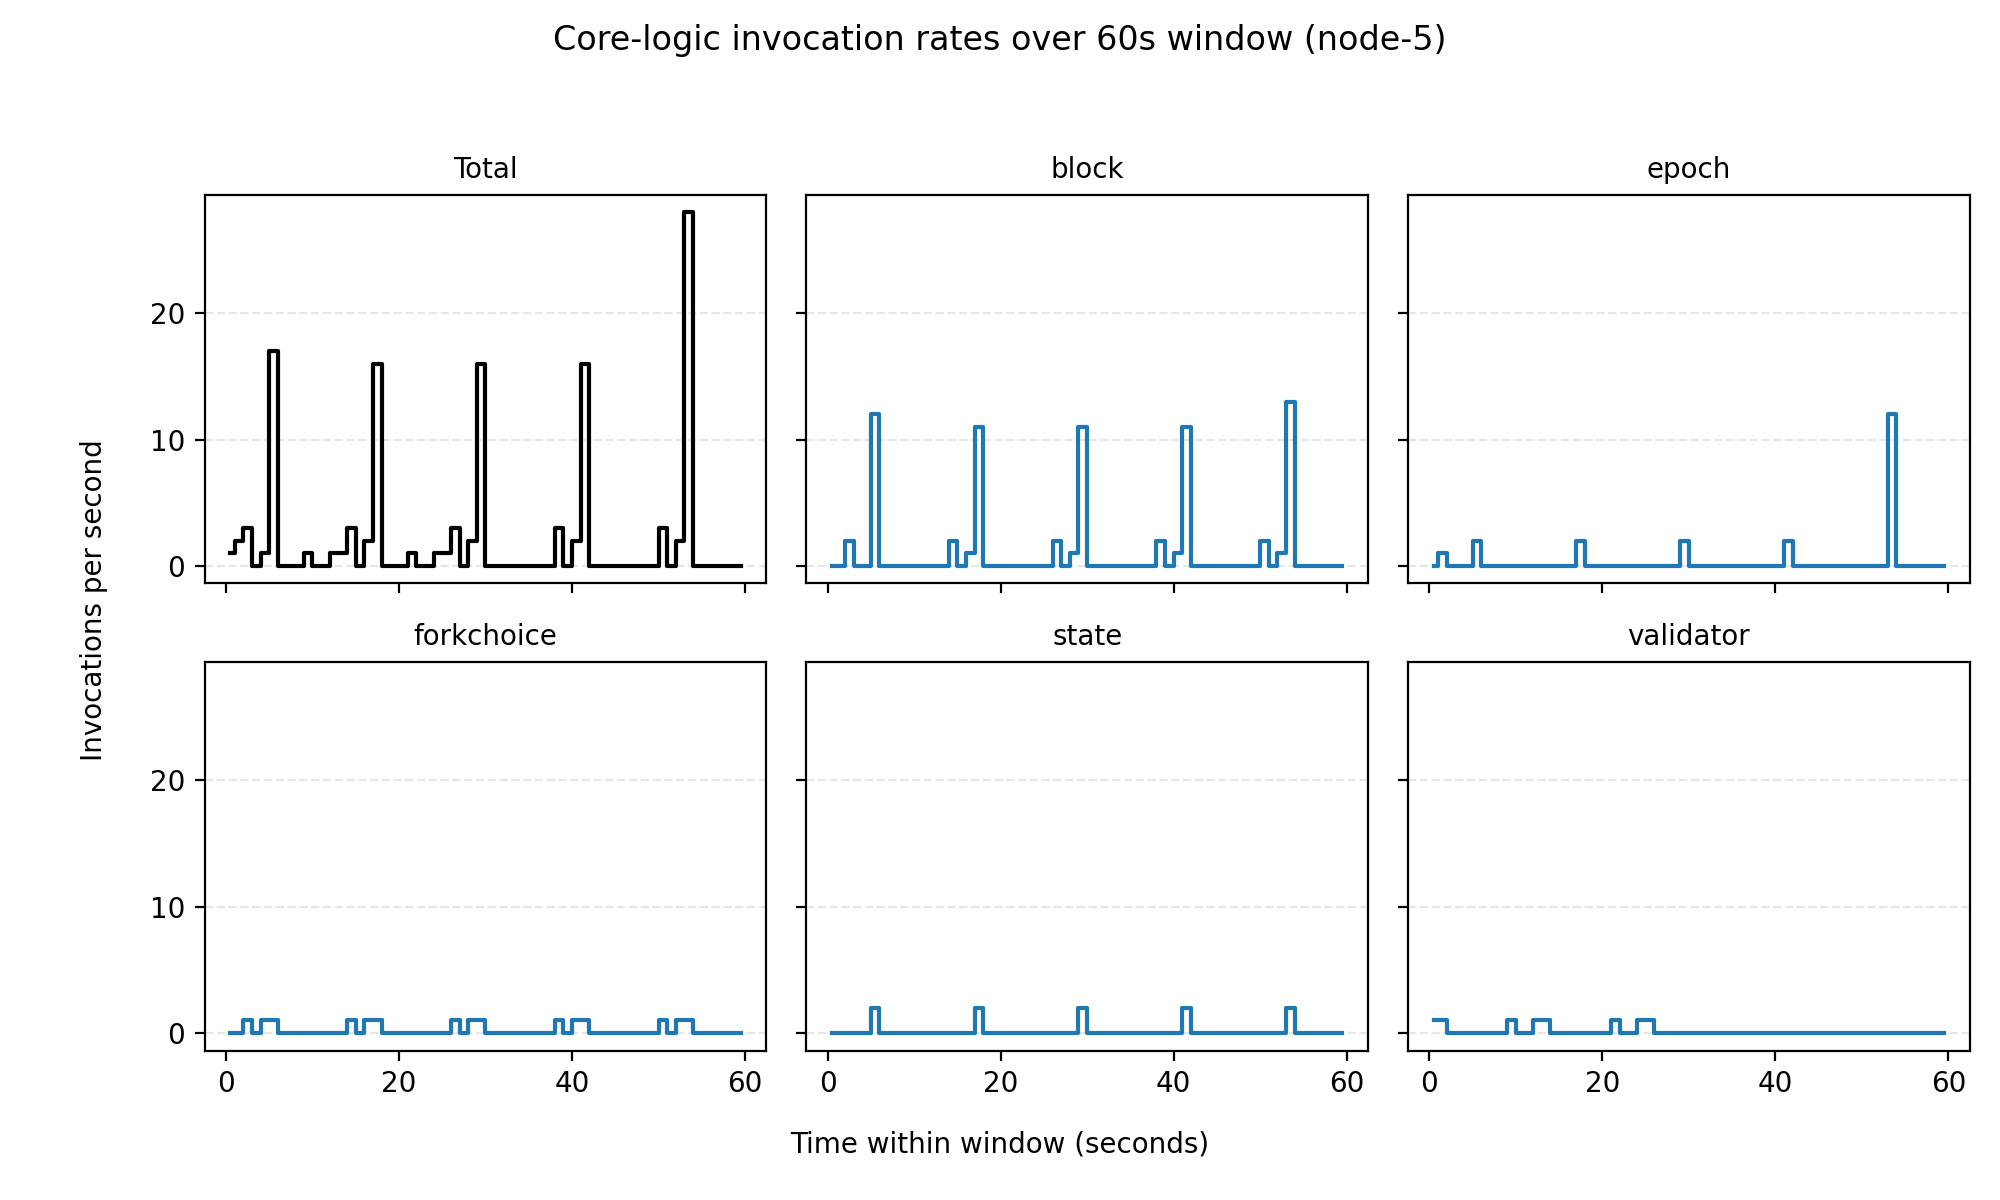
\includegraphics[width=\linewidth]{Figs/corelogic_node-5_60s_category_rates}
    \caption{Normal PoS testnet (no fuzzing).}
    \label{fig:corelogic_60s_normal}
  \end{subfigure}
  \hfill
  \begin{subfigure}{0.49\textwidth}
    \centering
    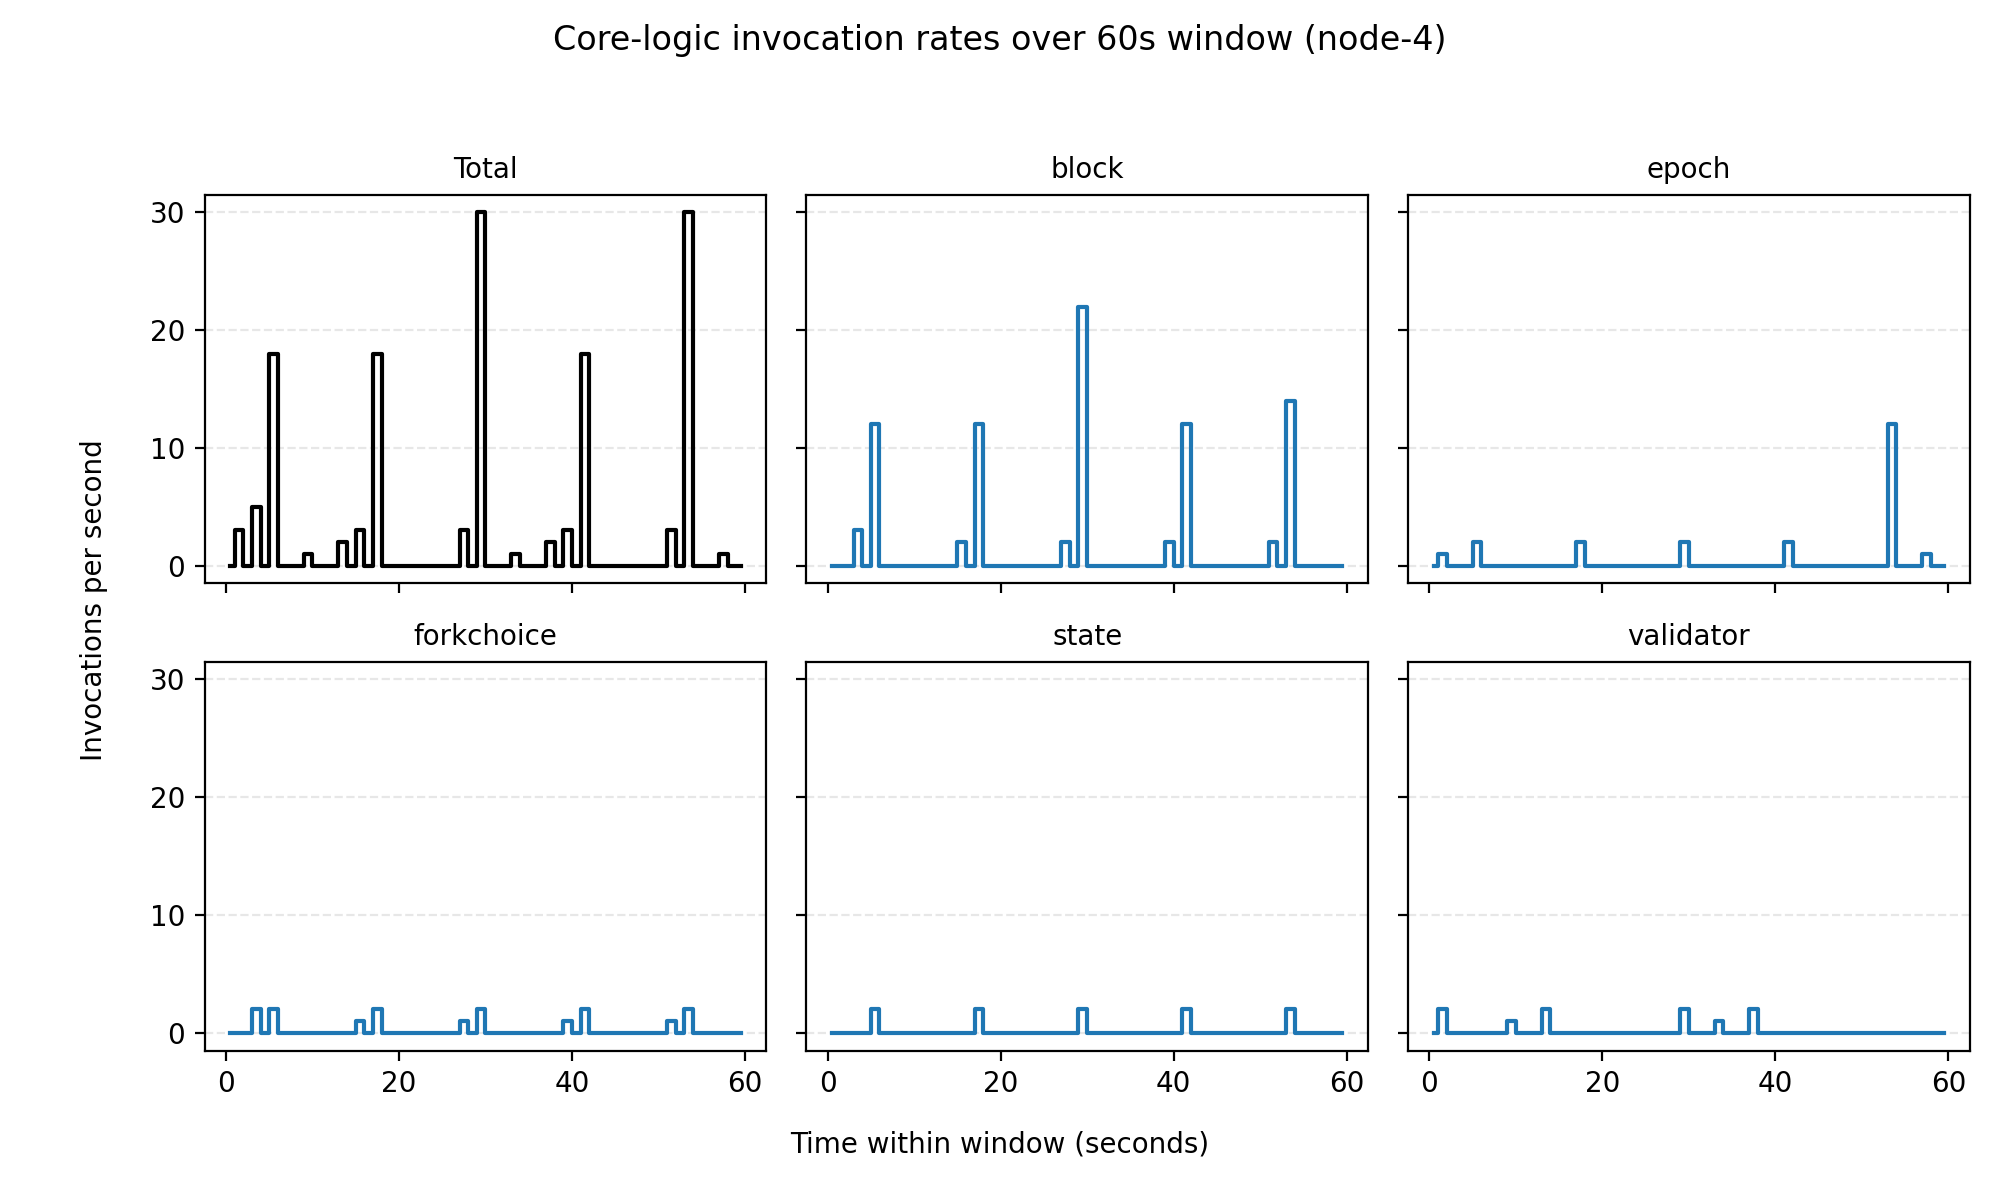
\includegraphics[width=\linewidth]{Figs/corelogic_node-4_60s_category_rates}
    \caption{PoS testnet under migrated PoW fuzzer.}
    \label{fig:corelogic_60s_fuzz}
  \end{subfigure}
  \caption{Comparison of core-logic invocation rates over 60-second windows on an Ethereum normal PoS testnet (a) and under fuzzing (b). Each panel shows the number of calls per second; most bins are empty, and activity is concentrated around slot boundaries. Validator duties are assigned probabilistically, so a node may be fully idle in some slots.}
  \label{fig:corelogic_60s_normal_vs_fuzz}
\end{figure*}

\subsection{The Core Logic Execution}
\label{subsec:sparsity}

In this section, we empirically characterize the invocation frequency of core logic functions in our instrumented testnet. The testnet follows the configuration in Section~\ref{subsec:corelogic}: each slot lasts \textbf{12 seconds}, and each epoch consists of \textbf{5 slots}, i.e., a full epoch spans \textbf{60 seconds}. 
This shortened epoch length is chosen for experimental convenience. It does not aim to reproduce mainnet epoch frequency exactly; rather, it preserves the slot/epoch heartbeat and the timing-gated structure of the consensus state machine that our analysis targets.
Figure~\ref{fig:corelogic_60s_normal} shows, for a randomly selected beacon node, the invocation rates of core-logic functions over a contiguous 60-second window (i.e., one full epoch), sampled at one-second resolution. 
The top-left panel reports the \emph{total} number of core-logic calls per second, while the remaining panels break this total down into the four categories defined in Section~\ref{subsec:corelogic} (block/data processing, epoch/schedule processing, forkchoice processing, and validator logic), together with the state-transition entry points. 

Two properties are immediately visible. 
First, the total series is dominated by a small number of sharp spikes aligned with slot boundaries, while the majority of one-second bins contain \emph{no} core-logic invocations at all. This directly reflects that conventional testnets advance protocol time in real time: between two slot ticks, the node mostly waits.
Second, the epoch/schedule panel exhibits a highly regular pattern---exactly one slot-advancing call every 12 seconds---whereas block, fork-choice, and validator panels show much sparser activity, reflecting that blocks and validator duties occur only in a subset of slots and are themselves gated by the protocol clock.

Our measurements confirm that, on a small eight-node testnet, the consensus core logic is executed in brief bursts at discrete temporal boundaries, while the system spends most wall-clock time waiting for the next scheduled or event-driven transition. 
This extreme sparsity is precisely what motivates our event-driven testnet design: by advancing time directly from one core-logic event to the next, we can eliminate idle intervals and dramatically increase the rate at which the consensus state machine is exercised.


\subsection{Low Effectiveness of Message-Driven Testing}
\label{subsec:fuzzing_limitation}

The sparsity and periodicity documented above critically limit the effectiveness of message-driven testing techniques, such as stateful consensus fuzzing and chaos testing, when applied to PoS testnets.
In these settings, the feedback-producing parts of consensus core logic are often time-triggered (slot/epoch). Therefore, even if a tester can generate or mutate network messages at a high rate, the testnet still cannot increase the density of core-logic execution beyond the real-time slot/epoch cadence, resulting in low effectiveness on core-logic testing.
Much of the testing budget is thus spent \textit{waiting} (for the next tick) or stressing only p2p surfaces, rather than \textit{exercising} the consensus state machine.

To validate this intuition, we ported a message-driven testnet consensus fuzzer, \textsc{LOKI}~\cite{ma2023loki} (originally designed for message-driven PoW-style testnets), to our PoS Ethereum testnet and reused its open-source harness and mutation strategies with minimal changes.
Message mutation is a natural strategy for protocols where most progress is driven by message arrivals; in such settings, a fuzzer can often increase effectiveness simply by increasing the rate and diversity of inputs.
However, in Ethereum PoS, a substantial portion of core logic cannot be triggered by messages alone: it additionally depends on protocol-defined time scheduling (slot/epoch ticks) and randomized duty assignment.
As a result, message-driven fuzzing strategies do not provide stable or dense feedback from consensus core logic on PoS testnets unless they are made aware of protocol time.

To support our analysis, we then ran the fuzzer for 30 minutes on the same 8-node, 16-validator setup and collected core-logic invocation statistics in exactly the same way as in the normal run. 
Figure~\ref{fig:corelogic_60s_normal_vs_fuzz} compares the per-category and total invocation rates over a 60-second window on a representative beacon node: the normal testnet in panel~(a) versus the fuzzing-enabled testnet in panel~(b). 
Although fuzzing injects additional inputs and perturbs network traffic, the overall shape of the curves remains almost unchanged: activity is still concentrated in sharp spikes around slot boundaries, the epoch/schedule panel continues to show a single clock tick every 12 seconds, and most one-second bins across all panels remain empty.

Besides the time-gating bottleneck, LOKI's message-driven strategy is also a poor fit for exercising Ethereum PoS data-processing core logic: it primarily injects \emph{extra} messages into the network rather than mutating and replaying \emph{valid} baseline messages under protocol constraints.
As a result, many injected messages fail decoding or validation checks and are dropped early, never reaching the deeper state-transition paths that constitute data-processing core logic.

This experiment demonstrates that simply migrating a PoW-oriented, message-driven testnet fuzzer to a PoS setting does not resolve the core-logic sparsity problem, and therefore does not substantially improve assurance about consensus correctness. At a high level, the reason is that the dominant bottleneck lies in the protocol’s time-driven schedule rather than in the availability of inputs: the fuzzer can inject or mutate blocks, attestations, and messages, but it cannot accelerate the slot/epoch heartbeat or compress the long idle intervals enforced by PoS timing.
We do not claim that all fuzzing strategies are ineffective for PoS; rather, our result shows that message-driven fuzzing transfers poorly unless the testing framework itself can control protocol time. More broadly, a consensus fuzzer can meaningfully exercise time-gated core logic only if it actively \emph{fits} the protocol's timing mechanism, rather than spending most of its effort perturbing p2p surfaces. This observation motivates the time-decoupled testnet framework that we present next and suggests a path toward future timing-aware fuzzing.